\newpage
\hypertarget{remCard tex}{}
\subsection{Implementing removeCard}
\texHeader

\disclaimerForTextualSyntax

\begin{itemize}

\itemWithRightTriangle Open \texttt{Partition.eclass}, go to the
\texttt{removeCard} signature and add a pair of curly brackets so that it looks like a proper method declaration. This entire scope can be referred to as the method's \emph{activity}, where the control flow (imperative top-layer) of a
transformation is defined.

\itemWithRightTriangle Complete the activity with a single pattern and return statement as depicted in Listing~\ref{eclipse:remCardDec}. Don't forget -- you
can use eMoflon's auto-complete feature here! Press \texttt{Ctrl + Space} on an
empty line, then select the pattern template to establish \texttt{deleteSingleCard}.

\itemWithRightTriangle Note that in this context, the \texttt{`\$'} operator indicates a \emph{ParameterExpression}%
\define{Parameter\-Expression}. This expression implicitly refers to parameters from arguments which are assigned by the operation. In \texttt{removeCard}'s case, the returned parameter refers to the \texttt{card} parameter.

\vspace{0.5cm}

\lstinputlisting[style=eclass, firstline=12, lastline=16, firstnumber=12, label=eclipse:remCardDec,caption={Control flow for \texttt{removeCard}}] {../03_removeCard/texRemCode/Partition.txt} 

\itemWithRightTriangle It should be mentioned that MOSL limits method definitions exclusively to the method's control flow. All actual transformation
rules are modelled in separate \emph{pattern} files. In this case, \texttt{removeCard}'s link deletion will be modelled in \texttt{[deleteSingleCard]}.

\vspace{0.5cm}

\itemWithRightTriangle Save \texttt{Partition.eclass}. An error should immediately appear below the editor. In the ``Problems'' tab, the message
states that the builder cannot find the specified pattern file (Fig.~\ref{eclipse:errorMissingPattern}). Well, this makes sense. You haven't created it yet! Click this message and press \texttt{Ctrl +
1} to invoke a ``Quick Fix'' dialogue (Fig.~\ref{eclipse:quickFix}). It offers to create a pattern file for you. Given that's exactly what you'd like, select the
option and press \texttt{Finish}.

\vspace{0.5cm}

\begin{figure}[htp]
	\centering
	\subfloat[The errors because of the missing pattern]{	
		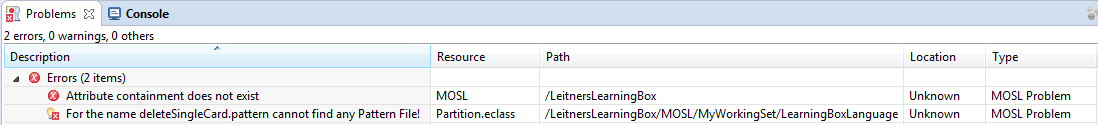
\includegraphics[width=1\textwidth]{eclipse_errorMissingPattern}
		\label{eclipse:errorMissingPattern}
	}
	\vspace{0.5cm}
	\subfloat[A quick fix to a missing pattern error]{
		  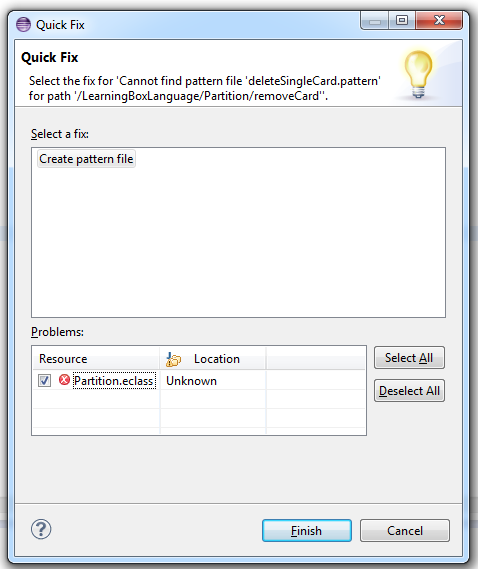
\includegraphics[width=0.45\textwidth]{eclipse_patternQuickFix}
		  \label{eclipse:quickFix}
	}
	\caption{Missing pattern error handling}
\end{figure}

\vspace{0.5cm}

\itemWithRightTriangle Alternatively, you can create a new folder with the name of the operation, in this case \texttt{removeCard} and create the \texttt{deleteSingleCard} pattern with the wizard.


\begin{figure}[htp]
	\centering
	\subfloat[Menu to create a pattern manually]{	
		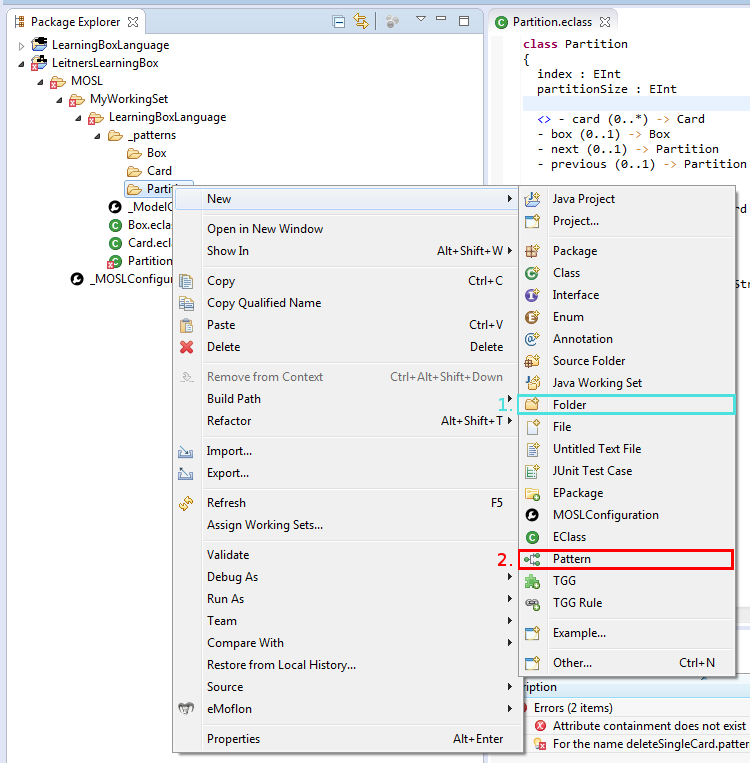
\includegraphics[width=0.9\textwidth]{eclipse_newFolderPatternMenu}
		\label{eclipse:newFolderPattern}
	}
	
	\subfloat[Wizard to create the \texttt{remove\-Card} folder]{	
			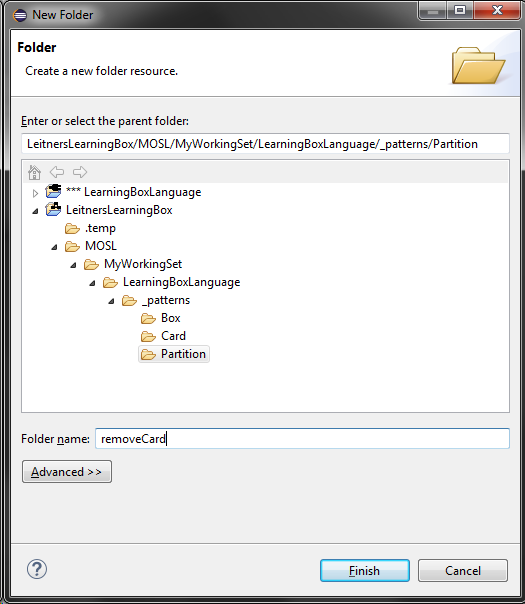
\includegraphics[width=0.45\textwidth]{eclipse_newFolder}
			\label{eclipse:newFoldern}
	}
	\subfloat[Wizard to create the \texttt{delete\-Single\-Card} pattern]{
		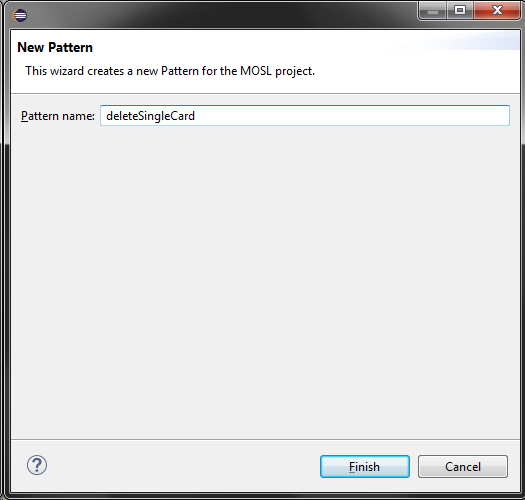
\includegraphics[width=0.45\textwidth]{eclipse_newPattern}
		\label{eclipse:newPattern}
	}
	\caption{Manual way to create a pattern}
\end{figure}

\newpage


\itemWithRightTriangle The new file will open in the editor, and you'll be able to see a new directory structure under ``LearningBoxLanguage/\_patterns''
(Fig.~\ref{eclipse:pattStruct}). To explain, \texttt{deleteSingleCard.pattern} is invoked by the method \texttt{removeCard}, which is in the \texttt{Partition}
EClass. \texttt{Partition} will eventually contain a folder for each method that uses a pattern.

\vspace{0.5cm}

\itemWithRightTriangle The content of any pattern file is simply a list \emph{object variable scopes}, and then,
within such a scope, operations such as `delete/create/find' this outgoing reference. Remember - the main goal of SDMs is to focus here is not on \emph{how},
but \emph{what}.

%\newpage

\begin{figure}[htp]
\begin{center}
  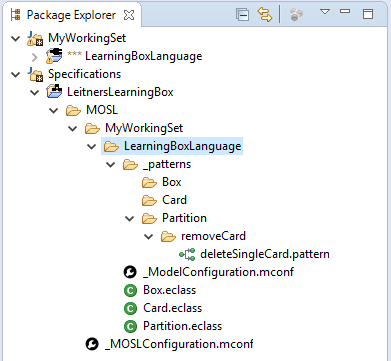
\includegraphics[width=0.6\textwidth]{eclipse_patternStructure}
  \caption{Directory structure for a pattern}
  \label{eclipse:pattStruct}
\end{center}
\end{figure}

\itemWithRightTriangle Create two object variables, \texttt{{\color{VIOLET}@this} : Partition}~and \texttt{@card : Card}\\ (Listings~\ref{eclipse:remCardDeleteSC}, Line~\ref{eclipse:remThisPartition} and~\ref{eclipse:remCardPartition}). When working with MOSL patterns, \texttt{`@'} indicates a \emph{ObjectVariableExpression}\define{ObjectVariable\-Expression}. This expression implicitly refers to object variables from the preceding story node.It also indicates that the variable is \emph{bound}. \texttt{{\color{VIOLET}this}} is bound to the object whose method is invoked, while \texttt{card} is bound to the value of the parameter with the same name. 

\vspace{0.5cm}

\itemWithRightTriangle Object variable scopes determine the changes to be applied to the any exiting references of the variable. Therefore, add:
\syntax{\color{RED}-- -card-> card} to \texttt{{\color{VIOLET}@this}} to destroy the \texttt{card} reference targeting the \texttt{card} object. Your pattern should now resemble Listing~\ref{eclipse:remCardDeleteSC}, Line~\ref{eclipse:remThisPartition}. 


\vspace{0.5cm}


\lstinputlisting[style=pattern, label=eclipse:remCardDeleteSC,caption={Object variables for \texttt{removeCard} and destroy the link between a card and its partition}] {../03_removeCard/texRemCode/deleteSingleCard.txt}

\vspace{0.5cm}

\itemWithRightTriangle In summary, any \emph{outgoing link
 variable}\define{Outgoing~Link Var\-i\-able} follows this syntax:

\syntax{[action]`-'nameOfOutgoingLV`-> 'targetOV\\
\\
With:\\
action := `{\color{RED}--}' | `{\color{GREEN}++}' | `!' | `!.'index\\
index := NUM\\
nameOfOutgoingLV := STRING\\
targetOV := STRING
}

\itemWithRightTriangle If you ever need to quickly remind yourself of specific reference or attribute names, press \texttt{alt} and the \texttt{left}
arrow to jump back from your pattern to your EClass. Conversely, to quickly open
or jump to a pattern, hover over the pattern name while holding \texttt{Ctrl}
until it's underlined, then click!

\itemWithRightTriangle Remember, links between classes can be specified as \emph{bidrectional EReferences},\footnote{Technically two
\emph{unidirectional EReferences}. Refer to Part II, Section 2.5.} linked together as opposites in ``LearningBoxLanguage/\_Mod\-el\-Config\-uration.mconf.'' In this case,
therefore, we don't need to worry about declaring \texttt{\color{RED}--
-cardContainer-> Card} inside \texttt{card}, as it would be redundant.

\itemWithRightTriangle Save and build your metamodel. If any errors occur, double check and make sure your activity and pattern match ours. 

\itemWithRightTriangle To see how the same method is crafted in the visual syntax, check out Fig.~\ref{ea:sdm_complete_control_flow} from the previous
section.

\end{itemize}
